% Capítulo 2
\chapter{Capítulo 2}

Este é o primeiro capítulo da parte central do trabalho, isto é, o desenvolvimento, a parte mais extensa de todo o trabalho. Geralmente o desenvolvimento é dividido em capítulos, cada um com subseções e subseções, cujo tamanho e número de divisões variam em função da natureza do conteúdo do trabalho.

Em geral, a parte de desenvolvimento é subdividida em quatro subpartes:

\begin{itemize}
   \item \textit{contextualização ou definição do problema} -- consiste em descrever a situação ou o contexto geral referente ao assunto em questão, devem constar informações atualizadas visando a proporcionar maior consistência ao trabalho;
   \item \textit{referencial ou embasamento teórico} -- texto no qual se deve apresentar os aspectos teóricos, isto é, os conceitos utilizados e a definição dos mesmos; nesta parte faz-se a revisão de literatura sobre o assunto, resumindo-se os resultados de estudos feitos por outros autores, cujas obras citadas e consultadas devem constar nas referências;
   \item \textit{metodologia do trabalho ou procedimentos metodológicos} -- deve constar o instrumental, os métodos e as técnicas aplicados para a elaboração do trabalho;
   \item \textit{resultados} -- devem ser apresentados, de forma objetiva, precisa e clara, tanto os resultados positivos quanto os negativos que foram obtidos com o desenvolvimento do trabalho, sendo feita uma discussão que consiste na avaliação circunstanciada, na qual se estabelecem relações, deduções e generalizações.
\end{itemize}

É recomendável que o número total de páginas referente à parte de desenvolvimento não ultrapasse 60 (sessenta) páginas.

\section{Seção 1}

Teste de figura:

\begin{figure}[htb]
	\centering
  	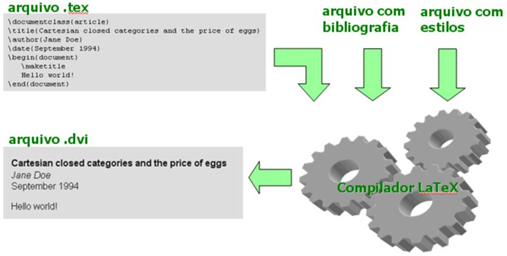
\includegraphics[scale=0.75]{Imagens/FiguraTeste.png}
  	\textsf{\caption{Teste de uma figura em formato .png}}
  	\label{fig:FiguraTeste}
\end{figure}


\section{Seção 2}

Referenciamento da figura inserida na seção anterior: \ref{fig:FiguraTeste}


\section{Seção 3}

Seção 3


\section{Seção 4}

Seção 4